\section{Method}
\label{sec:method}

\subsection{Notation and Shared Pipeline}
\label{sec:pipeline}

Let \(\mathcal{G}=(\mathcal{V},\mathcal{E})\) be a graph with node feature
matrix \(\mathbf{X}\in\mathbb{R}^{n\times d_{\mathrm{in}}}\) and adjacency
structure \(\mathbf{A}\). Given a dataset
\(\mathcal{D}=\{(\mathcal{G}_i,y_i)\}_{i=1}^{N}\), the objective is to learn
\(f_{\theta}:\mathcal{G}\rightarrow \hat{y}\), where \(\hat{y}\) is the predicted
graph label. Let \(B\) be the number of branches and \(L\) the number of
message-passing layers, and write the hidden state at branch \(b\) and layer
\(\ell\) as \(\mathbf{H}^{(\ell)}_{b}\), with \(b\in\{1,\ldots,B\}\). A
branch-local propagation step is
\begin{equation}
\mathbf{Z}^{(\ell)}_{b} =
\phi^{(\ell)}_{b}\left(\mathbf{H}^{(\ell-1)}_{b}, \mathbf{A}\right),
\label{eq:prop}
\end{equation}
where \(\phi\) is one of four standard operators: GCNConv \cite{kipf2017gcn},
GATConv \cite{velivckovic2017graph}, SAGEConv \cite{hamilton2017inductive}, or
GINConv \cite{xu2019gin}. The residual-enhanced update is
\begin{equation}
\mathbf{H}^{(\ell)}_{b} =
\mathbf{Z}^{(\ell)}_{b} +
\sum_{(b',\ell')\in\mathcal{N}(b,\ell)}
\mathcal{R}_{(b',\ell')\rightarrow(b,\ell)}
\left(\mathbf{H}^{(\ell')}_{b'}\right).
\label{eq:update}
\end{equation}
Only the residual neighborhood \(\mathcal{N}(b,\ell)\) and the residual
transform \(\mathcal{R}\) change across architectures. After the final layer,
each branch is pooled to a graph-level vector by global mean pooling, and the
branch vectors are combined before classification with a cross-entropy loss. We
deliberately avoid architecture-specific pooling heads such as differentiable
pooling~\cite{ying2018hierarchical}, because the goal is to isolate residual
topology rather than to compare readout mechanisms.
Fig.~\ref{fig:architecture} summarizes the shared pipeline and the compared
residual routes. The four operators were chosen as canonical representatives of
spectral-style convolution, attention-based aggregation, neighborhood sampling
and aggregation, and injective multiset aggregation.

\begin{figure}[!t]
\centering
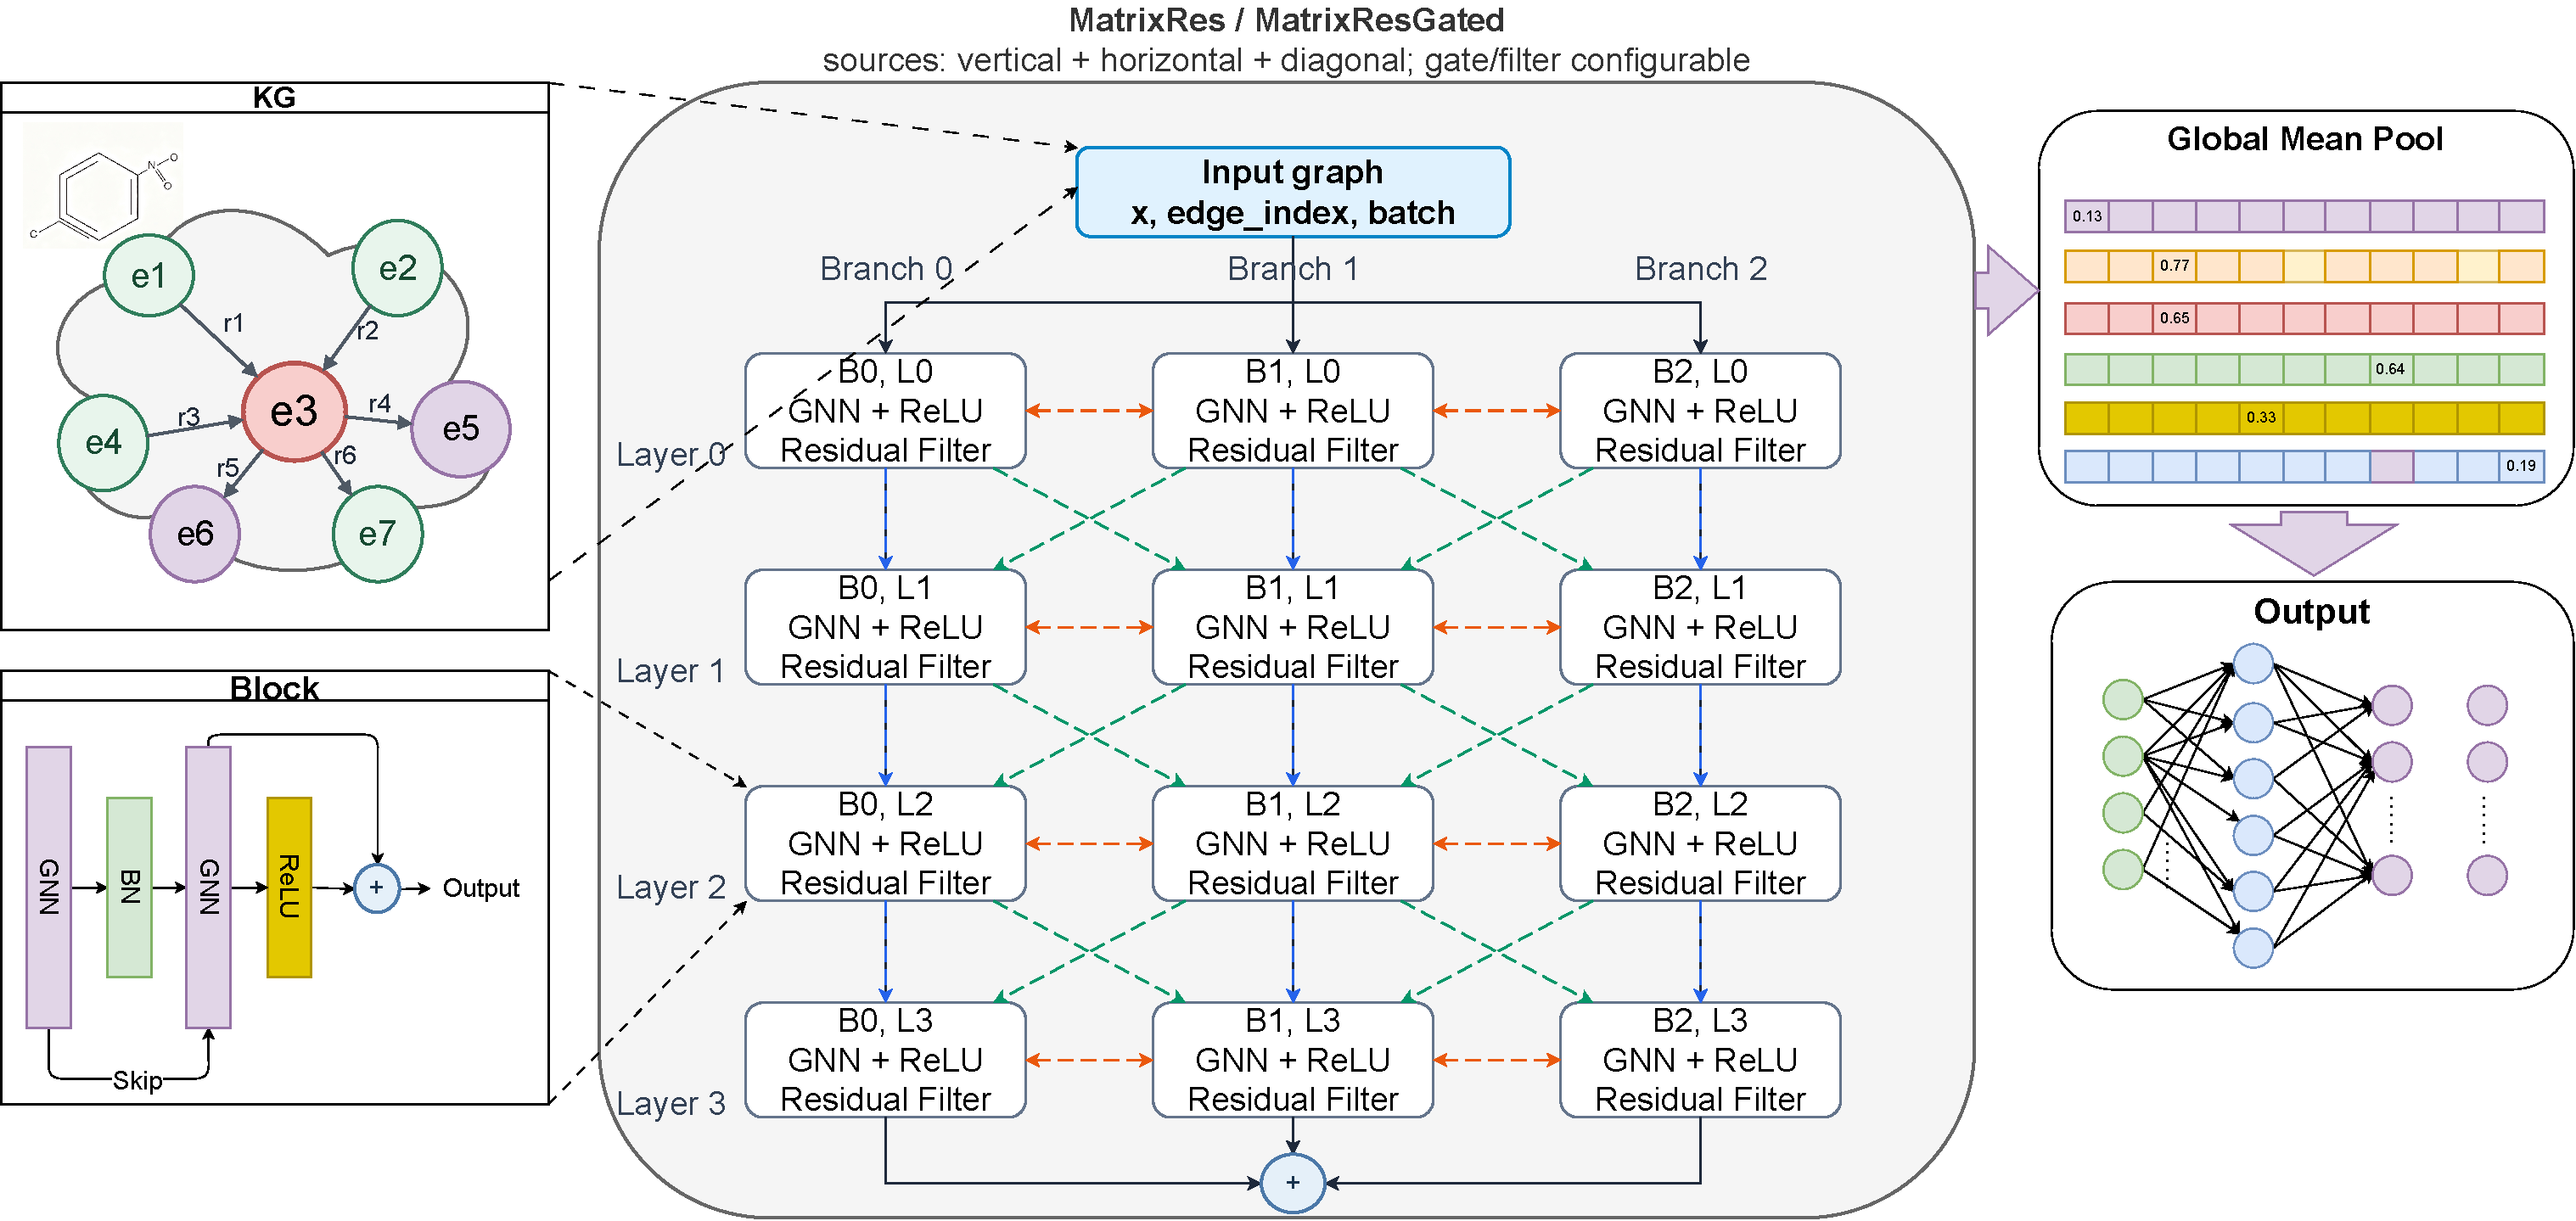
\includegraphics[width=0.95\columnwidth]{figures/cr_gnn_graph_architecture.pdf}
\caption{Compared residual neighborhoods on the branch-by-layer grid; the
backbone and graph-level readout are held fixed while the residual routes
change.}
\label{fig:architecture}
\end{figure}

\subsection{Residual Neighborhoods}
\label{sec:model}

\textbf{Plain} has no residual neighborhood, \(\mathcal{N}(b,\ell)=\emptyset\).
\textbf{VerticalRes} injects the previous layer of the same branch,
\(\mathcal{N}(b,\ell)=\{(b,\ell-1)\}\). \textbf{HorizontalRes} exchanges
information across adjacent branches at the same depth,
\(\mathcal{N}(b,\ell)=\{(b-1,\ell),(b+1,\ell)\}\), with boundary branches using
only valid neighbors; when \(B=1\) this neighborhood is empty. \textbf{MatrixRes}
combines vertical, horizontal, and diagonal neighbors:
\begin{equation}
\mathcal{N}(b,\ell)=
\{(b,\ell-1),(b-1,\ell),(b+1,\ell),(b-1,\ell-1),(b+1,\ell-1)\}.
\label{eq:matrix}
\end{equation}
This local stencil is intentionally not dense all-to-all mixing: it preserves an
interpretable residual structure over the branch-by-layer grid. Invalid boundary
neighbors are removed, so when \(B=1\), MatrixRes keeps the same-branch vertical
path after the first layer but has no branch-neighbor routes.

\textbf{MatrixResGated} uses the same neighborhood but controls the injected
signal through the residual transform:
\begin{equation}
\mathcal{R}(\mathbf{U}) =
\begin{cases}
\alpha \mathbf{U}, & \text{identity filtering with a gate},\\[2pt]
\alpha\,\mathrm{softshrink}_{\lambda}(\mathbf{U}), & \text{sparse filtering with a gate}.
\end{cases}
\label{eq:gate}
\end{equation}
Plain, VerticalRes, HorizontalRes, and MatrixRes use identity residual
filtering. MatrixResGated uses sparse filtering with \(\lambda=0.05\) and a
learnable scalar gate initialized at 0.8; when \(B=1\) it still applies gated
sparse filtering to the remaining matrix-residual paths. Top-\(k\) filtering and
fixed gates are supported but are not used for the reported results.

\subsection{Experimental Setup}
\label{sec:setup}

The main benchmark uses six TUDataset collections~\cite{morris2020tudataset}
accessed through PyTorch Geometric~\cite{fey2019fast}: PROTEINS, DD, ENZYMES,
MUTAG, AIDS, and Mutagenicity. PROTEINS and DD are binary protein-structure
tasks, ENZYMES is six-class, and MUTAG, AIDS, and Mutagenicity provide
molecular-graph robustness checks. Graphs are loaded with their provided
features; no handcrafted descriptors, augmentation, or edge rewiring are used,
so that the comparison reflects residual topology rather than feature
engineering.

All results use graph-level five-fold evaluation. For fold \(k\), test accuracy
is \(\mathrm{Acc}_{k}=|\mathcal{T}_{k}|^{-1}\sum_{(\mathcal{G}_{i},y_{i})\in\mathcal{T}_{k}}
\mathbf{1}[\hat{y}_{i}=y_{i}]\), and we report the mean over folds together with
the fold-level standard deviation. Accuracy is the primary metric because every
benchmark has discrete graph labels. For the synthetic benchmark we additionally
report macro-F1, which weights each class equally, and chance-normalized
accuracy, \(\mathrm{NAcc}=(\mathrm{Acc}-1/C)/(1-1/C)\), because raw accuracy is
not comparable across class counts. Mechanism metrics such as branch diversity,
cosine similarity, centered kernel alignment (CKA), residual activity, and
gradient norm are used as diagnostics, not as optimization targets.

To test residual topology under controlled structural granularity we add a
synthetic benchmark over five graph families: Bernoulli random graphs (ER),
Barab\'asi--Albert (BA) graphs, stochastic block models
(SBM)~\cite{holland1983stochastic}, Watts--Strogatz (WS)
graphs~\cite{watts1998collective}, and a regular-degree control. For each family
we generate seven datasets with \(C\in\{2,\ldots,8\}\) classes, 200 graphs per
class, and 30--80 nodes per graph. Node features are eight-dimensional vectors
derived from normalized degree and random channels; they do not encode the
label. Labels are controlled by family-specific structural parameters: edge
probability for ER~\cite{gilbert1959random}, preferential-attachment count for
BA~\cite{barabasi1999emergence}, within- and between-block probabilities for
SBM, rewiring probability for WS, and fixed degree for the regular control.
These families serve as stress tests, not as replacements for real benchmarks.

Table~\ref{tab:hyperparams} lists the shared settings. Models are optimized with
Adam~\cite{kingma2014adam}, and the checkpoint with the lowest validation loss
is retained for test evaluation.
Branch-count ablations
evaluate \(B=1,\ldots,8\) for HorizontalRes, MatrixRes, and MatrixResGated on
PROTEINS and DD under GCNConv. Sensitivity scans run on fold 0 at \(B=3\),
varying learning rate, dropout, hidden dimension, sparsity strength, and gate
initialization; selected candidates are then rerun across all five folds.
Experiments ran on an Ubuntu server with an AMD Ryzen 7 5700X CPU and an NVIDIA
RTX 3090 GPU.

\begin{table}[!t]
\centering
\caption{Key Experimental Settings}
\label{tab:hyperparams}
\footnotesize
\begin{tabular}{@{}p{0.38\columnwidth}p{0.58\columnwidth}@{}}
\toprule
Parameter & Value \\
\midrule
Operators & GCNConv, GATConv, SAGEConv, GINConv \\
Branches / layers & \(B=3\); \(L=4\) (DD: \(L=3\)) \\
Hidden dimension & 64 \\
Evaluation & Five-fold graph classification \\
Plain/Vertical/Horizontal & 200 epochs, patience 60, lr 0.005, wd \(10^{-4}\), dropout 0.5 \\
MatrixRes/MatrixResGated & 240 epochs, patience 80, lr 0.003, wd \(5\times10^{-5}\), dropout 0.3 \\
Schedule & ReduceLROnPlateau, factor 0.5, patience 15, min lr \(10^{-5}\) \\
Gradient clipping & Norm 2.0 \\
\bottomrule
\end{tabular}
\end{table}
